\documentclass{article}

\usepackage{textcomp} % for apostrophe

% for tables
\usepackage{multirow} 
\usepackage{array}
\newcolumntype{L}[1]{>{\raggedright\let\newline\\\arraybackslash\hspace{0pt}}m{#1}}
\usepackage{caption}

\title{Airbnb's New User Bookings Kaggle Competition}
\author{Lisa Oshita}

\usepackage{Sweave}
\begin{document}
\Sconcordance{concordance:final_report.tex:final_report.Rnw:%
1 13 1 1 0 285 1}


\maketitle

% -----------------------------------------------------------------------------------------------
\section{About the Competition}


Founded in 2008, Airbnb is an online accommodation marketplace featuring millions of houses,
rooms and apartments for rent or lease in over 200 countries. As part of a recruiting competition,
Airbnb partnered with Kaggle to host a data science competition starting in November 2015 and ending
in February 2016. The task of this competition was to build a model to accurately predict where new
Airbnb users will make their first bookings. Participants were given access to six data sets containing
information about the users and the 12 possible destinations to predict: US, France, Canada, United Kingdom, 
Spain, Italy, Portugal, Netherlands, Germany, Australia, Other and No Destination Found (NDF). No destination 
found indicates that a user did not make a booking. Other indicates that a booking was made to a 
country not already listed. 

% -----------------------------------------------------------------------------------------------

\section{XGBoost, Random Forest, Stacked Models}

Extreme Gradient Boosting (XGBoost) is a fairly new method of supervised learning that performs consistently 
better than single-algorithm models. It is a form of gradient boosting that introduces a different, more 
formal form of regularization to prevent overfitting---enabling it to outperform other models. Additionally, 
XGBoost algorithms are fast. At its core, the algorithm is parallelizable which allows this model to fully 
utilize the power of computers. As XGBoosts have been used to place highly in Kaggle competitions and were 
also used by many of the top 100 participants of this Airbnb competition, this was the model I first decided 
to explore and implement. 

The second model I decided to implement was a random forest. Random forests are another form of ensemble 
modeling that have performed well in Kaggle competitions. 

As the top three winners of this Airbnb competition used a form of stacked modeling, I also decided to 
explore a general form of this. Stacking, also called meta ensembling, is a technique used to combine 
information from individual predictive models to create a new model. Stacked models usually outperform 
its base models, as they are able to correct and build upon the performance of those base models. 

% -----------------------------------------------------------------------------------------------

\section{Exploratory Analysis}

Of the six available data sets, I focused on two: train\_users, which contains user information starting
in 2010, and sessions, which contains information about user\textquotesingle s web session activities. 

The sessions data contained 1,048,575 rows and 12,994 unique users. To minimize computation time when working 
with this data, 10\% of the rows from each unique user was randomly sampled. This new sampled data, containing 104,424 
rows, was used for all following analyses and model building. Figure blah shows the first six rows of the
sampled sessions data. 
% include head of train_users and sessions 

The train\_users data contained 213,415 rows and 16 original columns. Figure blah shows the first six rows 
of this data. Exploratory analysis of this data revealed several factors. 

\begin{table}[ht]
\centering
\begin{tabular}{| l |l |}
  \hline
  \textbf{Destination} & \textbf{Percentage of Bookings} \\ 
  \hline
  NDF & 58.35\% \\ 
  US & 29.22\% \\ 
  other & 4.73\% \\ 
  FR & 2.35\% \\ 
  IT & 1.33\% \\ 
  GB & 1.09\% \\ 
  ES & 1.05\% \\ 
  CA & 0.67\% \\ 
  DE & 0.50\% \\ 
  NL & 0.36\% \\ 
  AU & 0.25\% \\ 
  PT & 0.10\% \\ 
   \hline
\end{tabular}
\caption{Percentage of Bookings Made to Each Destination}
\label{table:countries}
\end{table}

Table \ref{table:countries} highlights how imbalanced the target classes, or destinations, are. NDF and US
account for almost 90\% of the entire data, indicating that a majority of users either 
have yet to make a booking, or book to locations in the US. The remaining nine, under-represented 
destinations make up less than 5\% of the data each.  

% Figure shows growth in accounts created over time
\begin{figure}[!htbp]
  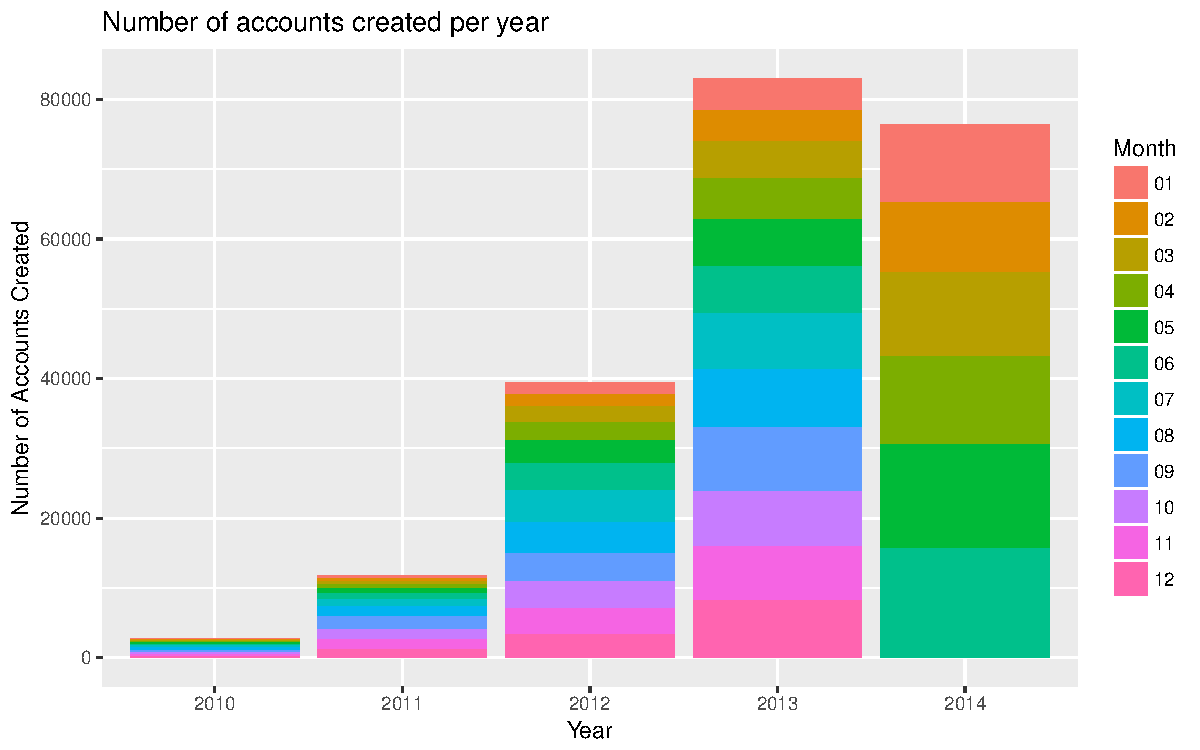
\includegraphics[scale = 0.5]{accountscreated.pdf}
  \caption{Number of accounts created each year (data only up to June 2014)}
  \label{fig:acct_created}
\end{figure}

% Bookings made over time 
\begin{figure}[!htbp]
  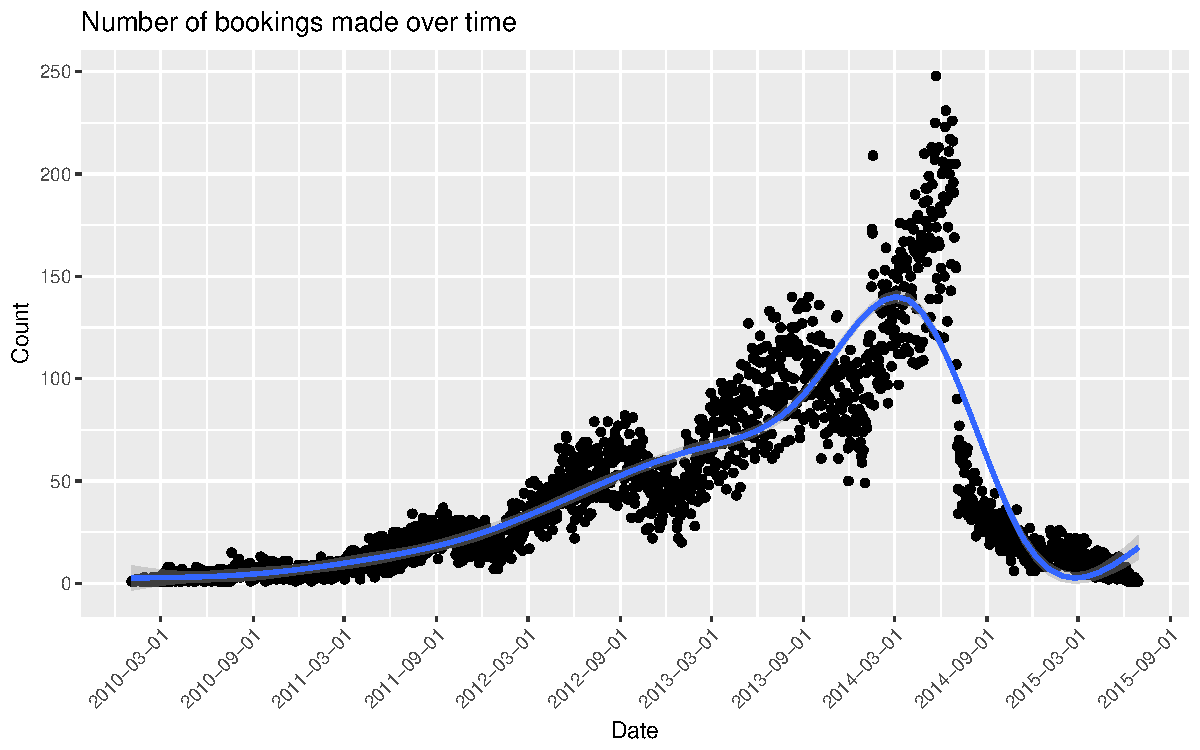
\includegraphics[scale=0.5]{bookingsovertime.pdf}
  \caption{Number of bookings made over time}
  \label{fig:bookings}
\end{figure}

Figure \ref{fig:bookings} and Figure \ref{fig:acct_created} depict the trends in the date features of
the train\_users data. Figure \ref{fig:acct_created} shows the huge increase in accounts created each year. 
The data only includes up to June 2014. 
depicts the trend in the number of bookings made from 2011 to 2015.
Interestingly, there seems to be a seasonality in the data. The number of bookings made seems to 
increase around September of each year. 



% include histogram of ages 
% include figure for genders 

Figure blah depicts the distribution of user's ages, after the age feature had been cleaned and 
missing values were handled with. The median age of all users was 36 years old. 

% -----------------------------------------------------------------------------------------------



\section{Feature Engineering}

From the train\_users data, 17 features were created. Date features were pulled apart into 
month, year, day of the week, and season features. The difference in days between each date feature 
(days between the date an account was created and the date of first booking, days between the date the 
user was first active and the date of first booking). Missing and erroneous values the gender feature 
were cleaned and recoded. The age feature contained several issues. 87,990 users (41\% of users) did 
not enter an age, while 2,345 users (1\% of users) entered an age of greater than 100. Erroneous values 
were cleaned and recoded, while missing values were filled in using an XGBoost model to predict those 
ages based on ages available in the data. 

From the sessions data, 320 features were created. The data was aggregated by each user and 
features counting the number of unique levels of each categorical feature were created. From secs\_elapsed, 
mean, median, standard deviation, minimum and maximums were calculated for each unique user. These features 
were then joined by user id to the train\_users data. 

\begin{table}[!htbp]
\centering
\begin{tabular}{|L{2cm}|L{10cm}|}
  \hline
  \multirow{9}{2cm}{\textbf{Original Features}} & Sign up method (facebook, basic, google) \\ \cline{2-2}
  & Sign up flow (integers 0 to 24) \\ \cline{2-2}
  & Language preference (25 options) \\ \cline{2-2}
  & Affiliate channel (direct, remarketing, api...) \\ \cline{2-2}
  & Affiliate provider (craigslist, bing, email-marketing...) \\ \cline{2-2}
  & First affiliate tracked (untracked, linked, local ops...) \\ \cline{2-2}
  & Sign up app (Web, Moweb, iOS, Android) \\ \cline{2-2}
  & First device type (Mac Desktop, iPad, iPhone...) \\ \cline{2-2}
  & First browser (Chrome, Firefox, Safari...) \\ \hline
  \multirow{5}{2cm}{\textbf{Derived Features}} & Year, month, day of the week, season features of date account created, 
  date first active, date first booking\\ \cline{2-2}
  & Days between date account created and date of first booking \\ \cline{2-2}
  & Days between date first active and date of first booking \\ \cline{2-2}
  & Age \\ \cline{2-2}
  & Gender \\ \cline{2-2} 
  & Count features created from the sessions data (number of times a user looked at recent reservations, number of 
  times a user looked at similar listings...) \\ \cline{2-2}
  & Mean, median, standard deviation, minimum, maximum of seconds elapsed for each user's web activity\\ \hline
\end{tabular}
\caption{Original and Derived Features included in the training data}
\label{table:features}
\end{table}

One-hot encoding was used to convert categorical features to a more machine learning compatible form.  
Essentially, a boolean column was generated for each level of a categorical feature. Continuous 
features were left as is. After one-hot encoding, there were a total of 596 features. Table 
\ref{table:features} displays all features, both originall and derived, 
that were included in the training data for model building. 


\section{Model Building and Results}

The method of building the XGBoost, random forest, and stacked model was more of a circular, iterative 
process in that, when new findings or discoveries were made, steps were retraced to implement or explore 
those possibilites. Nonetheless, the following describes the general process that was used to build the
three models. 

The full data was partitioned into one training set, containing 70\% of the full data (149,422 rows), and one 
test set containing 64,029 rows. All model building was performed on just the training set. For both the XGBoost 
and random forest models, five fold cross-validation was performed on the training set, including all 596 features. 
Both models achieved 87\% classification accuracy, as well as a Normalized Discounted Cumulative Gain (NDCG) score 
(the metric used in the actual competition) of 0.92. However, both models only made predictions for NDF, US, and 
other. Examining feature importance for each model showed that not all features were necessary. So, the models were 
refit to just the 200 most important features and cross-validation was performed again. While accuracy and NDCG
scores remained the same, computation time decreased tremendously. All following models were built only on just these 
200 features. 

\begin{table}[ht]
\centering
\begin{tabular}{| l | l | l |}
  \hline
  \textbf{Country} & \textbf{N} & \textbf{Proportion} \\ 
  \hline
  AU & 5670 & 0.05 \\ 
  CA & 5000 & 0.04 \\ 
  DE & 5944 & 0.05 \\ 
  ES & 6300 & 0.05 \\ 
  FR & 7034 & 0.06 \\ 
  GB & 6508 & 0.06 \\ 
  IT & 5955 & 0.05 \\ 
  NDF & 35000 & 0.30 \\ 
  NL & 5340 & 0.05 \\ 
  other & 7066 & 0.06 \\ 
  PT & 5320 & 0.05 \\ 
  US & 20000 & 0.17 \\ 
   \hline
\end{tabular}
\label{table:smote}
\end{table}

To account for the highly imbalanced classes, several over-sampling techniques were explored. Data for under-represented
destinations were over sampled with replacement and data from over-represented destinations were under sampled. 
Building and testing models on this new sampled training data resulted in worse predictive accuracy than previous
models. The final method settled on was Synthetic Minority Oversampling Techniques (SMOTE), in which underrepresented
classes are upsampled by with generated synthetic examples selected from the k-nearest neighbors of these under-represented 
destinations. This over-sampling technique was combined with undersampling of the over-represented destinations. The 
resulting training set contained 115,137 observations. Table \ref{table:smote} shows the number of observations and proportion
of data each destination accounts for, after SMOTE and undersampling was performed. 

The same model fitting processes (cross-validation with only the top 200 features) was again performed 
on this new training data. For both models, accuracy and NDCG scores remained the same. However, both models were 
able to make predictions for all countries (rather than just NDF, US and other), although predictions for these 
under-represented countries were not significantly accurate. Figures blah and blah show the confusion matrices of predictions
for the XGBoost and random forest fit to this new training data. Figures blah and blah display the feature importance 
for each model. 

% maybe include a visual explaining the flow of this stacked model 

Both models were then combined in a stacked model. The training data was partitioned into five folds, each 
fold making up around 20\% of the full training data. Each model was then built on the training folds, and 
tested on the held out fold. For example, the XGBoost was first built on folds one, two, three and four, and 
used to make predictions on fold five. In the second iteration, the XGBoost was build on folds two, three, 
four and five, and used to make predictions on fold one. This process was repeated for both models until each 
fold had been used as a test fold. Predictions from these models were stored as two columns in the training data. 
Then, each model was fit to the full training data (ignoring the folds and predictions created in the
previous step), and used to predict on the held out test set. Predictions from these models were stored in two 
columns in that test set. A final XGBoost was used as the model to combine, or stack the information from the 
previous processes. An XGBoost was fit to the predictions stored in the training set and tested on the predictions 
stored in the test set. Resulting accuracy and NDCG score for this stacked model was the same as its base models, 
as well as all previous models. 

\section{Discussion and Conclusion}

Although various strategies for improving model performance were explored, no effective strategy was found---each 
model achieved around 87\% accuracy and NDCG score of about 0.92. One 
explanation for this is how imbalanced the target classes are. As discussed above, two destinations make up
almost the entire data set, while the remaining 10 destinations each make up less than 5\% of the data each. 
Essentially, there is not enough information available about these under-represented destinations to enable each model 
to make predictions for those underrepresented countries. Instead, each model classified them mainly as bookings 
to the US. Since NDF and US constitute such a large portion of the data, the accuracy of each model 
remained fairly high at 87\%. In order to create a model that can make accurate predictions for all 12 possible 
destinations, a strategy to resolve this issue of highly imbalanced classes would need to be implemented.

To explain why the stacked model did not result in better performance, the base models need to be examined. 
Stacked models generally perform well when its base models differ in performance. For example, suppose base model 1
could predict five countries well, but not the other 7. Suppose base model 2 could predict those 7 countries well, 
but not the other 5. In this case, a stacked model would be useful because of its ability to build upon and 
correct each model's performance. But since both the random forest and XGBoost could only make accurate predictions 
for NDF and the US, the stacked model's performance was not a significant improvement. 

Possibilities for further work on this include stacking more models than just two. The top three participants of 
this competition combined numerous algorithms in multiple layers. Another possible strategy
to explore, used by the second place participant of this competition, is to build multiple models to predict 
and impute missing values for certain features. Missing or erroneous values was a significant issue with several 
features, like age and gender. Building models to address this may be helpful with model performance. One final possibility,
is to find a way to incorporate the other two available data sets: countries, which contains summary
statistics about the destinations, and  age\_gender\_bkts, which contains statistics describing the users' age group, 
gender, and destinations. One possible idea, as implemented by the second place winner, is to build models to 
predict features within the countries data set, and use those features in the final destination predictions. 


\section{References}



























\end{document}
